\chapter{Related Work}

In this section we explore some tools and techniques related to the activities described in our work. We have decided to divide this chapter into three sections: \textit{Product}, \textit{Process} and \textit{Automation}. 
Product describes \textit{Jenkins}, an alternative solution to the utilized automation tool (Team Foundation Server/Azure DevOps). Jenkins is one of the most popular applications for the implementation of continuous integration,delivery and deployment techniques and it constitutes an interesting object of study given its open source nature as opposed to the closed source approach taken by Microsoft with Azure DevOps. The completely customizable extensibility of Jenkins with the use of plugins is another characteristic that further motivated this initial comparison. 
Process elaborates on the concept of \textit{Behavior-Driven Development}, and on a possible tool (Cucumber) to employ said technique. We have decided to introduce the notion of BDD in order to describe a viable approach for the company to develop future applications with a major focus not only on the concept of testing, but also on the communication between developers, consultants and key users. This technique, while not directly utilized during the course of this project, may represents a key step for the improvement of the quality and quantity of testing techniques applied during a project development. Because of this reason, we believed it to be worthy of description. 
Finally, Automation gives some background information regarding the notion of \textit{Continuous Integration}. We decided to provide a brief introduction in this regard because of the fact that CI (and the related concepts of Continuous Deployment and Delivery) constitutes the basis for the employment of regression testing techniques which represent one of the final objectives of this work.

%********************************** %First Section  **************************************
\section{Product} 

Jenkins \cite{JenkinsGuide} is a java-based, open-source software initially created in order to automate the building and testing stages of the development process. The extreme flexibility of the tool made it adaptable to a very wide range of requirements such as version control, code quality monitoring, testing, build automation, etc.
The tool can be extended with the thousands of available open source plugins that that allow the implementation (and automation) of various DevOps tools and techniques. In this context Jenkins is seen as an \textit{orchestrator} tool.
Given its flexibility, Jenkins is primarily used to support Continuous Integration and Continuous Delivery approaches. Continuous Deployment is also achievable but often times more conservative procedures (such as a manual one-click deployment) are preferred by companies in order to have direct control over the process. A suite of related plugins that enables the use of CI/CD techniques is called a Jenkins Pipeline [Figure \ref{fig:jenkinsPipeline}]. Said pipelines are fundamentally a series of repeatable interlinked steps that may allow changes in the code to be automatically deployed. 
This chain of operations provides various benefits such as: Grouping of  multiple activities into clearly defined stages (if one of such stages fails, the process is interrupted), clear visibility of all aspects of the process and immediate feedback when problems arise.
Jenkins pipelines are composed by two kind of elements: \textit{stages} and \textit{steps}. A step is a minimal operation that tells the software to perform an action (like executing a script). A stage is a group of logically related sub-tasks (like building, testing, etc.). A machine executing a pipeline is called a \textit{Node}. Pipelines can be written directly in Jenkins or can be created in text files called \textit{JenkinsFile} where the single steps are defined.
Benefits of using said files include prevention of data loss (pipelines definitions are stored in the repository), code quality improvement (through code reviews) and security (access restrictions are the same as the ones used for the source code). The syntax used in these files may be declarative or scripted.


\begin{figure}[ht]
	\centering
	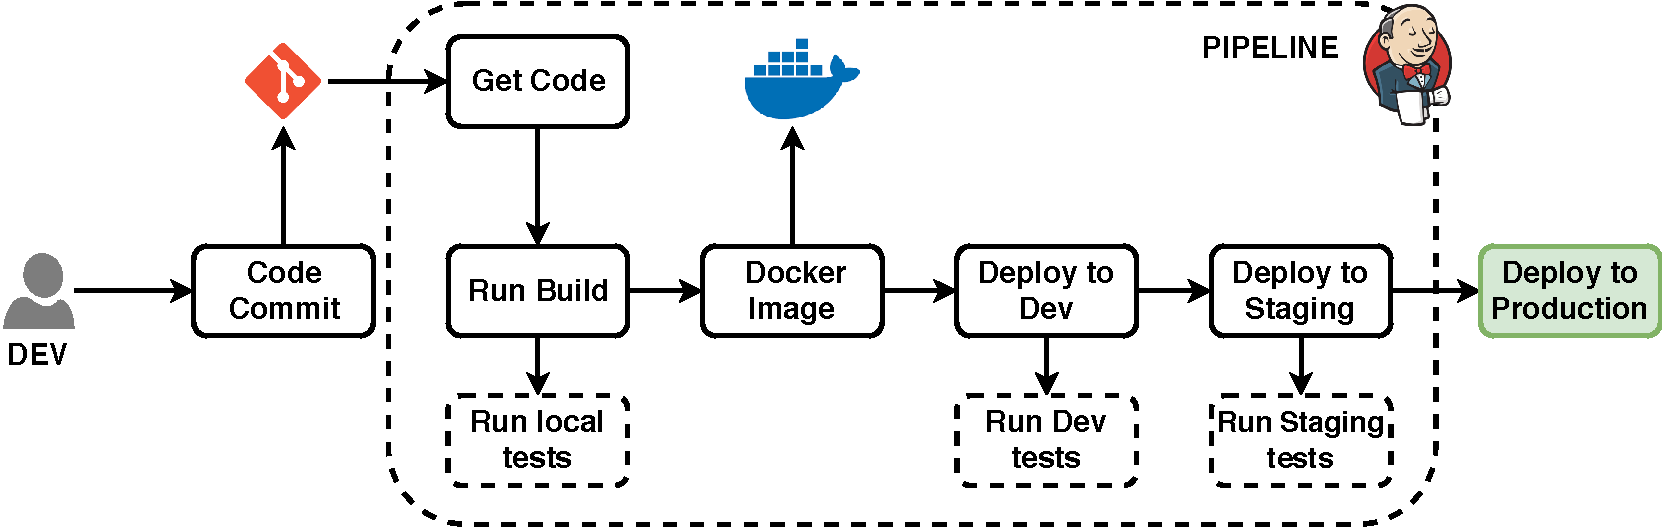
\includegraphics[scale=0.5]{Images/JenkisPipeline.pdf}
	\caption{Example of a Jenkins Pipeline}
	\label{fig:jenkinsPipeline}
\end{figure}

%********************************** %Second Section  **************************************
\section{Process} 

Behavior-Driven Development \cite{BDD} is a set of practices aimed at delivering high quality software while maintaining a stable stream of communication between developers, stakeholders and users. BDD tries to resolve the issues of Test-Driven Development and Acceptance Test-Driven Development by providing a better way for developers to understand scope and starting point of the testing activities that have to be performed on the application.
In the context of BDD, system specification are defined in a way that provides an high degree of understandability and automation capabilities. In order to make this possible a common (\textit{ubiquitous}) language is used (and understood) by all the parties involved in the development process.
BDD is started with the identification of the expected (or desired) behaviors of the application, which are then translated into a set of features. From this features user stories (that describe the interaction between user and system) are created together with their related scenarios (specific instances of a user story). The language used to present this scenarios allows to turn their (high level) description into executable specifications that will act as \textit{acceptance tests} that verify the behavior of the system (behavioral testing). This process is made possible by mapping each step of a scenario to specific portion of code that can then be executed as part of the acceptance test.
BDD also focuses on the readability of code which is seen as part of the project documentation. Because of this reason classes and methods names are usually self explanatory and allow the reader to understand what a specific portion of the code does without the need of additional information (this characteristic also affects the name and structure of unit tests).
Being an highly collaborative procedure (in which information regarding the system specifications are shared in plain English, or any other language of choice), BDD requires a way to define feature and scenarios while still maintaining a sufficient level of automation. A tool commonly used to implement such procedures is \textit{Cucumber} \cite{Cucumber}. Cucumber is a command-line tool that takes plain language text files (called \textit{feature files}), analyses them and runs them against the system. These files represent the previously mentioned executable specifications that tell the system \textit{what} to do. The features are described by concrete examples that use a common vocabulary understood by all parties. Said files are written using a syntax called \textit{Gherkin}. Gherkin enables software to derive meaning from plain language files by using a series of specific keywords. A Gherkin file [Algorithm \ref{alg:featureWithScenario}] is organized into:

\begin{enumerate}
  \item \textit{Feature}. To define some initial documentation regarding the purpose of the document.
  \item \textit{Scenario}. To describe the interaction with the system. A single feature comes with multiple scenarios that describe the expected reaction of the system in various situations. A Scenario is composed by a list of steps that have to be executed sequentially. It can either pass or fail and should be able to run on its own without the need of pre-existing data. Scenarios are divided into:
  \begin{itemize}
    \item Context. Defined by the keyword \textit{Given}. It declares the preconditions and prepares the environment.
    \item Event(s). Defined by the keyword \textit{When}, It represents the tested action(s) performed on the system.
    \item Outcome(s). Defined by the keyword \textit{Then}. It describes the expected outcome.
  \end{itemize}
  
  Each line of the scenario is known as a \textit{step}. Multiple steps can be concatenated using the keywords \textit{and} and \textit{but}.
\end{enumerate}

\begin{algorithm}[H]
\SetAlgoLined
\textbf{Feature}: Transfer Order\;
    \hspace{5mm} \textbf{Scenario}: Attempt a transfer without items\;
        \hspace{10mm} \textbf{Given} I have 0 Items in Warehouse\;
        \hspace{10mm} \textbf{When} I create a transfer order\;
        \hspace{10mm} \textbf{Then} an error message is prompted\;
\caption{A Feature with Scenario}
\label{alg:featureWithScenario}
\end{algorithm}


\textit{Step definitions} are portion of code that provide meaning to each feature step and that allow feature files to be executed. They are written in Ruby and tell the system \textit{how} to do something. All this definitions are usually bundled together in a single file. Cucumber scans the feature files looking for familiar patterns in order to map each step to the corresponding function declared in the step definition file. When a familiar pattern is found the associated code is executed. 
%********************************** %Third Section  **************************************
\section{Automation}

Continuous Integration \cite{CI} is a development practice that revolves around the frequent (daily, o even multiple times per day) merging and integration of code. Said technique is employed to increase the rate of release cycles and to improve quality, reliability and productivity. The starting point of CI techniques is keeping all the developed code for a given project in a single shared repository. This is usually achieved using some form of source control tool (like GIT) that the developers can use to access the source code, monitor changes and save modifications. Modern source control systems also allow the use of branches in order to work on various iterations of the product at the same time. Changes to the shared code are handled by a CI server [Figure \ref{fig:CI}] that performs an automated build of the software when changes are committed by the developers in order to detect potential error brought upon by the newly developed code (performing at least a daily or nightly build is usually considered a minimum requirement). An example of such tool is the previously seen Jenkins. Said server can also be used to complete an array of additional tasks (like testing, best practice checking, etc). A CI server is also capable of notifying the developers in case of an unsuccessful build or when problems occurs during the testing stages.

\begin{figure}[ht]
	\centering
	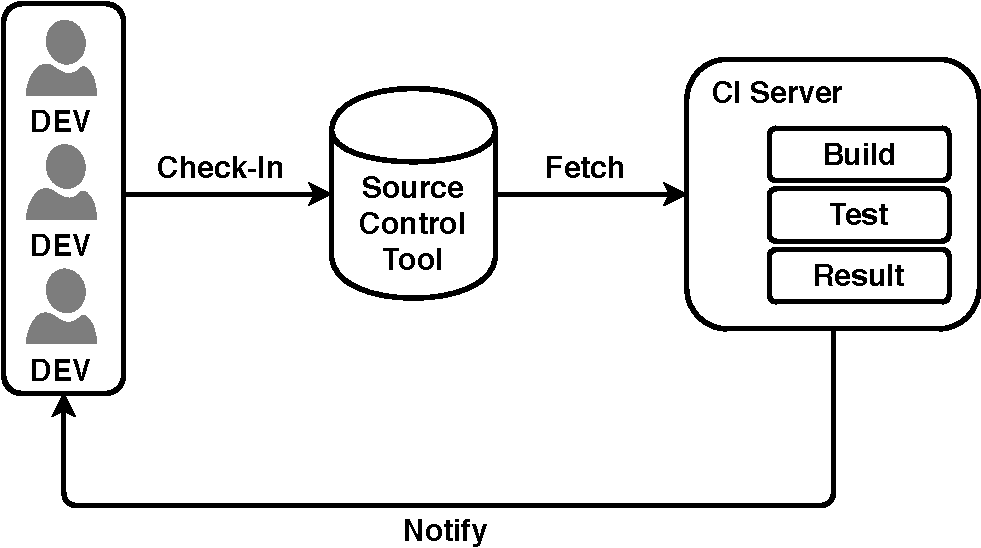
\includegraphics[scale=0.7]{Images/CI.pdf}
	\caption{Continuous Integration}
	\label{fig:CI}
\end{figure}

Although a successful build may already indicate some level of quality in the interested code, additional steps can be taken to further improve code reliability. Despite not being strictly a part of CI, continuous testing \cite{CT} is usually at least considered within the scope of such techniques and allows (thanks to the funtionalities offered by the CI server) the employment of various testing procedures, including (but not limited to):

\begin{itemize}
    \item Smoke Testing of the core product functionalities.
    \item Unit Testing of individual components (units) like functions, subroutines or methods. 
    \item Integration Testing of multiple software units (or components) interacting with each other that are tested to work as group.
    \item Acceptance Testing of the required usage scenarios to the determine to which degree the application meets the specified requirements.
\end{itemize}

The main advantage brought by the employment of CI techniques is naturally the automation of a series of processes that, if executed manually, would introduce the possibility of human error and be very time (and resource) consuming or even impossible to implement effectively during the whole development process. 